\documentclass[tikz,border=6pt]{standalone}
\usetikzlibrary{arrows.meta,shapes.geometric}
\begin{document}
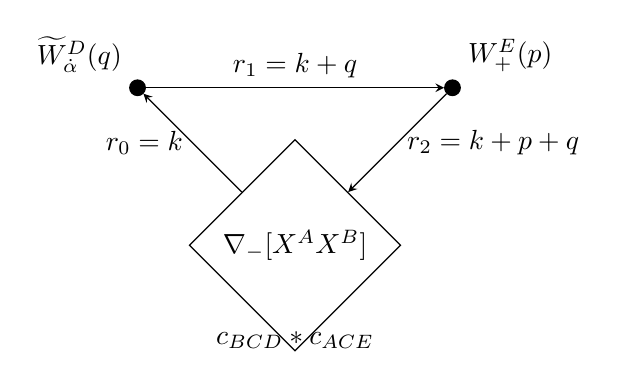
\begin{tikzpicture}[>=stealth]
\node[draw,diamond] (I) at (0,0) {$\nabla_-[X^A X^B]$};
\node[draw,circle,fill=black,inner sep=2pt,label=above left:$\widetilde W^D_{\dot\alpha}(q)$] (B) at (-2,2) {};
\node[draw,circle,fill=black,inner sep=2pt,label=above right:$W^E_+(p)$] (W) at (2,2) {};
\draw[->] (I) -- node[left] {$r_0=k$} (B);
\draw[->] (B) -- node[above] {$r_1=k+q$} (W);
\draw[->] (W) -- node[right] {$r_2=k+p+q$} (I);
\node at (0,-1.2) {$ c_{BCD}*c_{ACE} $};
\end{tikzpicture}
\end{document}
